% ch5-example.tex
\documentclass[../main/main]{subfiles}

\begin{document}

\chapter{応用例}
\footnotesize
ここでは本稿で学んだ特殊関数が具体的にどのように応用されているのかについて、
問題形式でいくつか紹介する。

\small
\section{Hermite多項式}

\Q{1}{1}{1次元調和振動子}

次の1次元調和振動子のSchr\"{o}dinger方程式について考える。
\begin{equation}\label{eq:Q1-1}
  \[ -\frac{\hbar^2}{2m} \dx{2} + \frac{1}{2} m\omega^2 x^2 \] \psi (x) = E \psi (x)
\end{equation}

\vspace{10pt}
(a). $\xi = \sqrt{\frac{m\omega}{\hbar}} x, \ \lambda= \frac{2E}{\hbar \omega}$ (ともに無次元量) とおくと
次のようになることを示せ。
\begin{equation}\label{eq:Q1-1(a)}
  \frac{d^2 \psi}{d \xi^2} + (\lambda - \xi^2) \psi = 0
\end{equation}

(b). 方程式\eqref{eq:Q1-1(a)}の解を$\psi =e^{-\frac{\xi^2}{2}} f(\xi)$とおくと
次のようになることを示せ。
\begin{equation}\label{eq:Q1-1(b)}
  \frac{d^2 f(\xi)}{d \xi^2} - 2\xi \frac{d f(\xi)}{d\xi} + (\lambda -1) f(\xi) = 0
\end{equation}

(c). 方程式\eqref{eq:Q1-1(b)}の解$f(\xi )$について、$\lambda-1 = 2n \ (n=0, 1, 2, \dots)$でないときは
$\psi =e^{-\frac{\xi^2}{2}} f(\xi)$が無限遠で発散してしまうので物理的に関心がない。
これより\eqref{eq:Q1-1(b)}はHermiteの微分方程式となり、
解は$f(\xi) = c_n H_n(\xi ) \ (c_n: 任意定数)$と書ける。
以上のことを整理して、方程式\eqref{eq:Q1-1}を満たす規格化された波動関数$\psi (x)$とエネルギー固有値$E$が
次のように求められることを示せ。
\begin{equation}
  \psi_n (x) = \sqrt{\frac{1}{2^n n!}} \( \frac{m \omega}{\hbar \pi } \)^{\frac{1}{4}}
	e^{-\frac{m\omega}{2\hbar} x^2} H_n \( \sqrt{\frac{m \omega}{\hbar}}\ x \),
	\qquad E_n = \( n+\frac{1}{2} \) \hbar\omega 
  \qquad (n=0, 1, 2, \dots)
\end{equation}


\section{Legendre関数}
\Q{2}{1}{静電場の多重極展開}

原点Oの近くの領域$V$内に静止した電荷分布$\rho (\bm{r}^\prime)$があるとき、
原点から十分離れた領域$V$外部の点$\bm{r}$においてはこの電荷分布による
静電ポテンシャル$\phi (\bm{r})$がどのように見えるか考えよう。
なお、電磁気学の理論により$\phi (\bm{r})$は次式によって与えられることが分かっている。
\begin{equation}\label{eq:Q2-1}
  \phi(\bm{r}) = \frac{1}{4\pi \epsilon_0} 
	\int_V \frac{\rho(\bm{r}^\prime)}{|\bm{r} - \bm{r}^\prime|} d^3 \bm{r}^\prime
\end{equation}

\vspace{10pt}
(a). $\bm{r}$と$\bm{r}^\prime$のなす角を$\theta^\prime$とする。
多重極展開により、\eqref{eq:Q2-1}が次のように書きなおせることを示せ。
\begin{equation}\label{eq:Q2-1(a)}
   \phi(\bm{r}) = \frac{1}{4\pi \epsilon_0} \sum_{n=0}^\infty \frac{1}{r^{n+1}}
	\int_V {r^{\prime}}^n P_n(\cos \theta^\prime) \rho (\bm{r}^\prime) \, d^3 \bm{r}^\prime
\end{equation}

(b). \eqref{eq:Q2-1(a)}の$n=0$の項は次のようになることを示せ。
\begin{align}
  &\phi_0(\bm{r}) = \frac{1}{4\pi \epsilon_0} \frac{q}{r} \\
	&全電荷 \ q \equiv \int_V \rho (\bm{r}^\prime) d^3 \bm{r}^\prime
\end{align}

(c). $n=1$の項は次のようになることを示せ。
\begin{align}
  &\phi_1(\bm{r}) = \frac{1}{4\pi \epsilon_0} \frac{\bm{r}\cdot\bm{p}}{r^3}  \\
	& 電気双極子モーメント \ \bm{p} \equiv \int_V \bm{r}^\prime \rho (\bm{r}^\prime) d^3 \bm{r}^\prime
\end{align}


(d). $n=2$の項は次のようになることを示せ。
\begin{align}
  &\phi_1(\bm{r}) = \frac{1}{4\pi \epsilon_0} \frac{3}{2} \frac{Q}{r^5} \\
	&\footnotesize 電気四重極モーメント \ Q \equiv 
		\int_V \[ (\bm{r}\cdot\bm{r}^\prime)(\bm{r}\cdot\bm{r}^\prime) - \frac{1}{3} (r r^\prime)^2 \]
		\rho (\bm{r}^\prime) d^3 \bm{r}^\prime 
\end{align}


\vspace{24pt}
\Q{2}{2}{球座標系の3次元Laplace方程式と球面調和関数}

3次元Laplace方程式$\Delta \psi = 0$を球座標系$(r, \theta, \varphi)$で解くことを考える。
球座標系での方程式は次のように書ける。
\begin{equation}\label{eq:Q2-2}
  \[ \frac{1}{r^2} \frac{\6}{\6 r} \( r^2 \frac{\6}{\6 r} \) 
	+ \frac{1}{r^2\sin\theta} \frac{\6}{\6\theta} \( \sin\theta \frac{\6}{\6\theta} \)
	+ \frac{1}{r^2\sin^2\theta} \frac{\6^2}{\6\varphi^2} \] \psi (r, \theta, \varphi) = 0
\end{equation}

\vspace{10pt}
(a). $\psi(r, \theta, \varphi) = R(r) \, \Theta (\theta) \, \Phi (\varphi)$とおいて
方程式\eqref{eq:Q2-2}を変数分離すると次のように書けることを示せ。
\begin{align}
  &\frac{d^2}{d \varphi^2} \Phi(\varphi) + m^2 \Phi(\varphi) = 0 \label{eq:Q2-2-phi}\\
  &\[ \frac{1}{\sin\theta} \frac{d}{d\theta} \( \sin\theta \frac{d}{d\theta} \) 
	+ \left\{ l(l+1) - \frac{m^2}{\sin^2\theta} \right\} \] \Theta(\theta) = 0 
		\label{eq:Q2-2-theta}\\
  &\[r^2 \dr{2} + 2r \dr{} - l(l+1) \] R(r) = 0 \label{eq:Q2-2-r}
\end{align}

(b). まず方程式\eqref{eq:Q2-2-phi}を解く。
解$\Phi(\varphi)$が方位角$\varphi$について1価となるためには
$\Phi(\varphi+2\pi) = \Phi(\varphi)$が必要である
\footnote{
このような条件は\textbf{周期境界条件}と呼ばれることがある。
}
。
この条件の下では、方位角$\varphi$について規格化された方程式\eqref{eq:Q2-2-phi}の基本解が
次のようになることを示せ。
\begin{equation}\label{eq:Q2-2-sol-Phi}
  \Phi(\varphi) = \frac{1}{\sqrt{2\pi}} e^{im\varphi} \qquad (m = 0, \pm1, \pm2, \dots)
\end{equation}

(c). 次に方程式\eqref{eq:Q2-2-theta}を解く。
これはLegendreの陪微分方程式であり、$m$が整数であるときに
解$\Theta(\theta)$が収束するためには、$l$が$|m| \leq l$を満たす整数でなければならないことが知られている。
またこのとき、基本解のひとつである(第1種)Legendre陪関数$P_l^m(\cos\theta)$はつねに収束し、
もうひとつの基本解である第2種Legendre陪関数$Q_l^m (\cos\theta)$は
$\theta=0, \pi$で発散することが分かっている
\footnote{
本来はこのことも確かめる必要があるが、ふつうはこの事実を認めてしまってかまわない。
}
。
このことから、天頂角$\theta$について規格化された方程式\eqref{eq:Q2-2-theta}の収束する基本解が
次のようになることを示せ。
\begin{equation}\label{eq:Q2-2-sol-Theta}
  \Theta(\theta) = \sqrt{\frac{2l+1}{2} \frac{(l-m)!}{(l+m)!}} \ P_l^m (\cos\theta) \qquad
	(-l \leq m \leq l)
\end{equation}
これまでに得られた解\eqref{eq:Q2-2-sol-Phi}, \eqref{eq:Q2-2-sol-Theta}の積をとって
位相因子$(-1)^m$をつけたものが球面調和関数$Y_{lm} (\theta, \varphi)$である。

\vspace{6pt}
(d). 最後に方程式\eqref{eq:Q2-2-r}を解く。
Eulerの方程式と呼ばれるこの方程式の基本解は$r^l, \ r^{-l-1}$となることを示せ。

\vspace{10pt}
以上のことから、球座標系の3次元Laplace方程式\eqref{eq:Q2-2}の収束する一般解は、
$l$に依存する任意定数$A_l, B_l$をもちいて次のように書ける。
\begin{equation}
  \psi(r, \theta, \varphi) 
	= \sum_{l=0}^\infty \sum_{m=-l}^l (A_l \, r^l + B_l \, r^{-l-1}) \ Y_{lm} (\theta, \varphi)
\end{equation}



\section{Laguerre多項式}
\Q{3}{1}{水素原子}

次の中心力場のSchr\"{o}dinger方程式を考える。
\begin{equation}\label{eq:Q3-1}
  \[ -\frac{\hbar^2}{2m} \Delta + V(r) \] \psi (r, \theta, \varphi) = E \psi (r, \theta, \varphi)
\end{equation}
ただし球座標系$(r,\theta, \varphi)$におけるラプラシアンは次の通りである。
\begin{equation}
  \Delta = \frac{1}{r^2} \frac{\6}{\6 r} \( r^2 \frac{\6}{\6 r} \) 
	+ \frac{1}{r^2\sin\theta} \frac{\6}{\6\theta} \( \sin\theta \frac{\6}{\6\theta} \)
	+ \frac{1}{r^2\sin^2\theta} \frac{\6^2}{\6\varphi^2}
\end{equation}

\vspace{10pt}
(a). $\psi(r, \theta, \varphi) = R(r) \, \Theta (\theta) \, \Phi (\varphi)$とおいて
方程式\eqref{eq:Q3-1}を変数分離すると次のように書けることを示せ。
\begin{align}
  &\frac{d^2}{d \varphi^2} \Phi(\varphi) + m^2 \Phi(\varphi) = 0 \label{eq:Q3-1-phi}\\
  &\[ \frac{1}{\sin\theta} \frac{d}{d\theta} \( \sin\theta \frac{d}{d\theta} \) 
	+ \left\{ l(l+1) - \frac{m^2}{\sin^2\theta} \right\} \] \Theta(\theta) = 0 
		\label{eq:Q3-1-theta}\\
  &\[\frac{1}{r^2} \dr{} \( r^2 \dr{} \) 
		+ \frac{2m}{\hbar^2} (E-V(r)) - \frac{l(l+1)}{r^2} \] R(r) = 0 \label{eq:Q3-1-r}
\end{align}

\eqref{eq:Q3-1-phi}と\eqref{eq:Q3-1-theta}は問題[2-2]で考えたLaplace方程式のときとまったく同じであるから、
解の$(\theta, \varphi)$依存性は球面調和関数$Y_{lm} (\theta, \varphi)$になる。

\vspace{10pt}
(b). 中心力場の特別な場合として水素様原子を考えよう
\footnote{
電子と陽子を1個ずつもつ水素原子に加え、
1個の電子と複数個の陽子からなる多価イオンをまとめて水素様原子と呼んでいる。
たとえば$\mathrm{He}^{+}$や$\mathrm{Li}^{2+}$などがそれに当たる。
}
。
以下では束縛状態(すなわち$r\to\infty$で$R(r)\to 0$となる場合)についてのみ議論することにする。

\vspace{6pt}
価数$Z$の原子核をもつ水素様原子のポテンシャルは次のように書ける。
\begin{equation}
  V(r) = - \frac{1}{4\pi\epsilon_0} \frac{Ze^2}{r}
\end{equation}
いま$R(r)$を
\begin{equation}
  R(r) = z^l e^{-\frac{z}{2}} f(z), \qquad
  z = 2\epsilon r, \qquad 
  \epsilon = \frac{\sqrt{-2mE}}{\hbar}
\end{equation}
と変数変換し、さらに定数$a_0$を
\begin{equation}
  a_0 = \frac{\hbar^2}{m} \frac{4\pi\epsilon_0}{e^2}
\end{equation}
と定義する
\footnote{
ここで導入した定数$a_0$は基底状態の水素原子の半径を意味しており、\textbf{Bohr半径}と呼ばれている。
その大きさは約$0.529$\AA である。
}
。
このとき方程式\eqref{eq:Q3-1-r}が次のように書き換えられることを示せ。
\begin{equation}\label{eq:Q3-1(b)}
  z f^{\prime\prime} (z) + (2l+2-z) f^{\prime} (z) + \( \frac{Z}{\epsilon a_0} -l-1 \)f(z) = 0
\end{equation}


(c). 方程式\eqref{eq:Q3-1(b)}はLaguerreの陪微分方程式であり、
その解は$\frac{Z}{\epsilon a_0}$が$0\leq l \leq \frac{Z}{\epsilon a_0}-1$をみたす整数であるときのみ
$z\to\infty$で$f(z)\to 0$となることが知られている。
そこで$n = \frac{Z}{\epsilon a_0}$とすると、
方程式\eqref{eq:Q3-1(b)}の解は規格化因子を除いて次のように書けることを示せ。
\begin{equation}
  f(z) = L_{n+l}^{2l+1} (z) \qquad
  \(
  \begin{array}{c}
    0\leq l \leq n-1 \\
    n= 1, 2, \dots
  \end{array}
  \)
\end{equation}


(d). エネルギー固有値$E$が次のように離散的な値のみ許されることを示せ。
\begin{equation}
  E_n = - \frac{Z^2 \hbar^2}{2m a_0^2} \frac{1}{n^2}  \qquad (n=1, 2, \dots)
\end{equation}


(e). Laguerre陪多項式の漸化式\eqref{eq:Lnk-req}および直交性\eqref{Lnk-chokko}を用いて
\begin{equation}
  \int_0^\infty x^{k+1} e^{-x} \[ L_n^k (x) \]^2 dx
	= (2n+1-k) \frac{(n!)^3}{(n-k)!}
\end{equation}
を確認し、規格化された固有関数$\psi(r, \theta, \varphi)$が次のようになることを示せ。
\begin{equation}
  \psi_{nlm}(r, \theta, \varphi)
	= \frac{2}{n^2} \( \frac{Z}{a} \)^\frac{3}{2}
		\sqrt{\frac{(n-l-1)!}{\[ (n+l)! \]^3}} 
		\( \frac{2Z}{n a_0}r \)^l e^{-\frac{Z}{n a_0} r} L_{n+l}^{2l+1} \( \frac{2Z}{n a_0}r \) 
		Y_{lm} (\theta, \varphi) 
\end{equation}



\section{Bessel関数}


\vspace{24pt}
\Q{4}{1}{円形開口のFraunhofer回折}

\vspace{-12pt}
\begin{figure}[H]
  \centering
  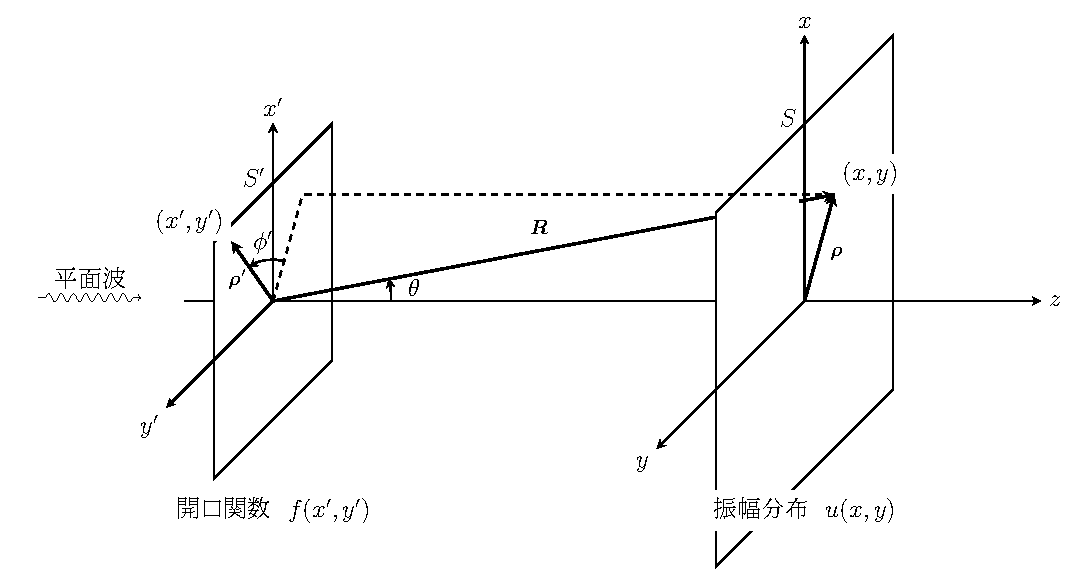
\includegraphics[width=120mm]{../TikZ/diffraction/diffraction.pdf}
  \caption{Fraunhofer回折の概念図}
  \label{fig:diffraction}
\end{figure}

図\ref{fig:diffraction}
のように$z$軸負方向から波数$k$の平面波が小さい平面開口$S^\prime$に入射すると回折現象が起こり、
後方のスクリーン$S$上に像ができる。
開口の中心$(x^\prime, y^\prime) = (0, 0)$からスクリーン$S$上の任意の点$(x, y)$までの距離$R$が
十分大きいとみなせる場合の回折は特別にFraunhofer回折と呼ばれ、
電磁気学の理論によればスクリーン$S$上の回折光の振幅分布$u(x, y)$が
次のように開口関数$f(x^\prime, y^\prime)$の2次元Fourier変換に比例することが知られている。
\begin{equation}\label{eq:Q4-1u(x,y)}
  u(x, y) \propto \iint_{S^\prime} f(x^\prime, y^\prime) e^{-ik(xx^\prime + yy^\prime)/R} 
	dx^\prime dy^\prime
\end{equation}


\vspace{12pt}
(a). 次の等式を示せ。
\begin{equation}
  \int_0^{2\pi} e^{-ix\cos\phi^\prime} d\phi^\prime = 2\pi J_0(x)
\end{equation}

(b). 開口$S^\prime$が半径$a$の円であるとき、開口関数$f(x^\prime, y^\prime)$は
\begin{numcases}
  {f(x^\prime, y^\prime) = }
    1 & $({x^\prime}^2+{y^\prime}^2 \leq a^2)$ \\
    0 & $({x^\prime}^2+{y^\prime}^2 > a^2)$
\end{numcases}
と書ける。スクリーン$S$の中心から$S$上の点$(x, y)$へ至るベクトルを$\bm{\rho}$、
開口$S^\prime$の中心から$S^\prime$上の点$(x^\prime, y^\prime)$へ至るベクトルを$\bm{\rho}^\prime$
とし、$\bm{\rho}$と$\bm{\rho}^\prime$のなす角を$\phi^\prime$としたとき、
$xx^\prime + yy^\prime = \bm{\rho}\cdot\bm{\rho}^\prime = \rho \rho^\prime \cos\phi^\prime $と書ける。
これを用いて円形開口の場合の\eqref{eq:Q4-1u(x,y)}を計算し、振幅分布$u(x, y)$が次のようになることを示せ。
\begin{equation}
  u(x, y) \propto \frac{2\pi aR}{k\rho} J_1 \( \frac{ka}{R} \rho \)
\end{equation}


\newpage

\Q{4}{2}{円型膜の振動}

半径が$a$の円型膜の振動について考える。
簡単のため円型膜の円周上は固定してあり、
時刻$t=0$において膜全体を高さ$h$だけ引っ張り上げて静止させるものと仮定する。
すなわち、次の偏微分方程式を考えることになる。
\begin{numcases}{}
  \textbf{波動方程式} & $\( \Delta - \dfrac{1}{c^2}\dfrac{\6^2}{\6 t^2} \) \psi (r, \theta, t) = 0$ 
		\label{eq:Q4-2-wave-eq}\\
  \textbf{境界条件} &  $\psi (a, \theta, t) = 0$ 
		\label{eq:Q4-2-boundary}\\
  \textbf{初期条件} &  $\psi (r, \theta, 0) = h, \quad \[ \dfrac{\6 \psi}{\6 t} \]_{t=0} = 0$
		\label{eq:Q4-2-first}
\end{numcases}
ここで$c$は膜の材質によって決まる正の定数である。
また$(r,\theta)$座標系におけるラプラシアンは次の通りである。
\begin{equation}
  \Delta = \frac{\6^2}{\6 r^2} + \frac{1}{r} \frac{\6}{\6 r} + \frac{1}{r^2} \frac{\6^2}{\6 \theta^2}
\end{equation}

\vspace{12pt}
(a). $\psi(r, \theta, t) = R(r) \Theta(\theta) T(t)$とおいて方程式\eqref{eq:Q4-2-wave-eq}を変数分離すると
次のように書けることを示せ。
\begin{align}
  &\frac{d^2}{d t^2} T(t) + c^2k^2 T(t) = 0 \label{eq:Q4-2(a)-1}\\
  &\frac{d^2}{d \theta^2} \Theta(\theta) + m^2 \Theta(\theta) = 0 \label{eq:Q4-2(a)-2}\\
  &\[ \dr{2} + \frac{1}{r} \dr{} + \( k^2-\frac{m^2}{r^2} \) \] R(r) = 0 \label{eq:Q4-2(a)-3}
\end{align}

\vspace{12pt}
(b). 方程式\eqref{eq:Q4-2(a)-3}は次数$m$についてのBesselの微分方程式であり、
基本解は$J_m(kr)$と$N_m(kr)$である。
しかし後者は$r\to 0$で発散し解として不適切なので捨てる。
いま$m$次のBessel関数の正の零点を小さい順に$\alpha_{m1}, \alpha_{m2}, \dots$とする。
$\Theta(\theta)$についての周期境界条件$\Theta(\theta+2\pi) = \Theta(\theta)$および
$r$についての境界条件\eqref{eq:Q4-2-boundary}を考慮すると、
定数$m$や$k$は次の値のみが許されることを示せ。
\begin{equation}
  k_{ml} = \frac{\alpha_{ml}}{a} \qquad
  \left(
  \begin{array}{c}
    m= 0, \pm1, \pm2, \dots \\
    l = 1, 2, \dots
  \end{array}
  \right)
\end{equation}
これより、境界条件\eqref{eq:Q4-2-boundary}を満たす
方程式\eqref{eq:Q4-2-wave-eq}の一般解は次のように書ける
\footnote{
ここで$m<0$は$m>0$の場合と従属になるので和に加えていない。
}
。
\begin{align}
  &\hspace{-36pt} \psi_{ml} (r, \theta, t) 
	= \sum_{m=0}^\infty \sum_{l=1}^\infty 
		\[ A_{ml} \cos\( \frac{c\, \alpha_{ml}}{a} t \) + B_{ml} \sin \( \frac{c\, \alpha_{ml}}{a}t \) \] 
		J_m \( \frac{\alpha_{ml}}{a} r \) \notag\\
  &\hspace{48pt}\times ( C_{ml}\cos m\theta + D_{ml}\sin m\theta )
\end{align}

\vspace{12pt}
(c). 初期条件\eqref{eq:Q4-2-first}を考慮すると、$m\geq 1$の項は不適切なので捨てられること、および
$m=0$における任意定数が次のように定まることを示せ。
\begin{equation}
  A_{0l}= \frac{2}{\alpha_{0l} J_1(\alpha_{0l})}, \qquad
  B_{0l} = 0, \qquad
  C_{0l} = h, \qquad
  D_{0l} = 0 
\end{equation}
これより、求める解は次のようになる。
\begin{equation}
  \psi_l (r, \theta, t)
	= \sum_{l=1}^\infty \frac{2h}{\alpha_{0l} J_1 (\alpha_{0l})}
	\cos\( \frac{c\, \alpha_{0l}}{a} t \) J_0 \( \frac{\alpha_{0l}}{a} r \)
\end{equation}

\vspace{12pt}
(d). 半径$a$の円型膜の代わりに、半径$a, b \ (a>b)$のふたつの同心円で囲まれた環状の膜の振動について
考えるとどうなるか説明せよ。初期条件により任意定数は確定しなくてよい。


\newpage
\Q{4}{3}{Airy方程式}

Airy方程式
\begin{equation}\label{eq:Q4-3}
  \frac{d^2y}{dx^2} - xy = 0
\end{equation}
の解は第1種変形Bessel関数$I_\nu (x)$とBessel関数$J_\nu (x)$で表せることが知られている。
このことを以下の手順にしたがって確認する。

\vspace{10pt}
(a). $x\geq 0$のとき、方程式\eqref{eq:Q4-3}を$\xi = \frac{2}{3}x^{\frac{3}{2}}$と変数変換すると
次のようになることを示せ。
\begin{equation}
  \frac{d^2 y}{d \xi^2} + \frac{1}{3\xi} \frac{d y}{d \xi} - y = 0
\end{equation}

(b). Bessel関数を使って解ける微分方程式の処方箋にしたがって、$x\geq 0$における\eqref{eq:Q4-3}の解が
次のように表せることを示せ。
\begin{equation}\label{eq:Q4-3(b)}
  y = \sqrt{x} \[ c_1 I_{\frac{1}{3}} \( \frac{2}{3}x^{\frac{3}{2}} \)
		+ c_2 I_{-\frac{1}{3}} \( \frac{2}{3}x^{\frac{3}{2}} \)  \] \qquad (x \geq 0)
\end{equation}

(c). 同様に$x\leq0$のとき$\zeta = \frac{2}{3} (-x)^\frac{3}{2}$と変数変換し、
解が次のように表せることを示せ。
\begin{equation}\label{eq:Q4-3(c)}
  y = \sqrt{-x} \[ c_3 J_{\frac{1}{3}} \( \frac{2}{3} (-x)^{\frac{3}{2}} \)
		+ c_4 J_{-\frac{1}{3}} \( \frac{2}{3} (-x)^{\frac{3}{2}} \)  \] \qquad (x\leq 0)
\end{equation}

\vspace{6pt}
Airy方程式\eqref{eq:Q4-3}の解\eqref{eq:Q4-3(b)}, \eqref{eq:Q4-3(c)}は
$x=0$で滑らかにつながることが期待される。
このことを要請して4つの任意定数を絞ることを考えよう。

\vspace{12pt}
(d). 上で得られた解\eqref{eq:Q4-3(b)}, \eqref{eq:Q4-3(c)}の導関数が次のようになることを示せ。
\begin{numcases}{y^\prime = }
    x \[ c_1 I_{-\frac{2}{3}} \( \frac{2}{3} x^{\frac{3}{2}} \) 
		+ c_2 I_{\frac{2}{3}} \(  \frac{2}{3} x^{\frac{3}{2}}\) \]
	& $(x>0)$ \\
    x \[ c_3 J_{-\frac{2}{3}} \( \frac{2}{3} (-x)^{\frac{3}{2}} \) 
		- c_4 J_{\frac{2}{3}} \(  \frac{2}{3} (-x)^{\frac{3}{2}}\) \]
	& $(x<0)$
\end{numcases}

(e). $x=0$において解が滑らかにつながるという要請から
$( すなわち \displaystyle \lim_{x\to +0} y = \lim_{x\to -0} y 
かつ \displaystyle\lim_{x\to +0} y^\prime = \lim_{x\to -0} y^\prime )$、
4つの任意定数の間に次の関係が成り立つことを示せ
\footnote{
  Bessel関数や変形Bessel関数の$x\to \pm0$極限を考える際はそれぞれの一般項を用いるとよい。
\vspace{4pt}
}
。
\begin{equation}
  c_3 = -c_1, \qquad \quad c_4 = c_2
\end{equation}

以上の議論から、Airy方程式\eqref{eq:Q4-3}の一般解は次のように求められる
\footnote{
\textbf{[参考]} \ 
実用上の観点から、一般解\eqref{eq:Q4-3-sol-1}, \eqref{eq:Q4-3-sol-2}
において$(c_1, c_2) = \( -\frac{1}{3}, \frac{1}{3} \), \ \( \frac{1}{\sqrt{3}}, \frac{1}{\sqrt{3}} \)$
とおいたものが広く用いられる。
前者はAiry関数 $\mathrm{Ai} (x)$(第1種Airy関数)、
後者はBiry関数$\mathrm{Bi} (x)$(第2種Airy関数)と呼ばれる。すなわち、
\begin{figure}[H]\footnotesize
\begin{minipage}{0.60\hsize}
\begin{align*}
  &\mathrm{Ai} (x) = \left\{
  \begin{alignedat}{2}
    &\frac{\sqrt{x}}{3} \[ - I_{\frac{1}{3}} \( \frac{2}{3} x^{\frac{3}{2}} \) 
		+ I_{-\frac{1}{3}} \(  \frac{2}{3} x^{\frac{3}{2}}\) \]
	& & (x\geq 0) \\
    &\frac{\sqrt{-x}}{3} \[  J_{\frac{1}{3}} \( \frac{2}{3} (-x)^{\frac{3}{2}} \) 
		+ J_{-\frac{1}{3}} \(  \frac{2}{3} (-x)^{\frac{3}{2}}\) \]
	&\quad &(x\leq 0) 
  \end{alignedat}
  \right. \\
  &\mathrm{Bi} (x) = \left\{
  \begin{alignedat}{2}
    &\sqrt{\frac{x}{3}} \[  I_{\frac{1}{3}} \( \frac{2}{3} x^{\frac{3}{2}} \) 
		+ I_{-\frac{1}{3}} \(  \frac{2}{3} x^{\frac{3}{2}}\) \]
	& & (x\geq 0) \\
    &\sqrt{\frac{-x}{3}} \[ - J_{\frac{1}{3}} \( \frac{2}{3} (-x)^{\frac{3}{2}} \) 
		+ J_{-\frac{1}{3}} \(  \frac{2}{3} (-x)^{\frac{3}{2}}\) \]
	&\, &(x\leq 0)
  \end{alignedat}
  \right.
\end{align*}
\end{minipage}
\hfill
\begin{minipage}{0.45\hsize}
  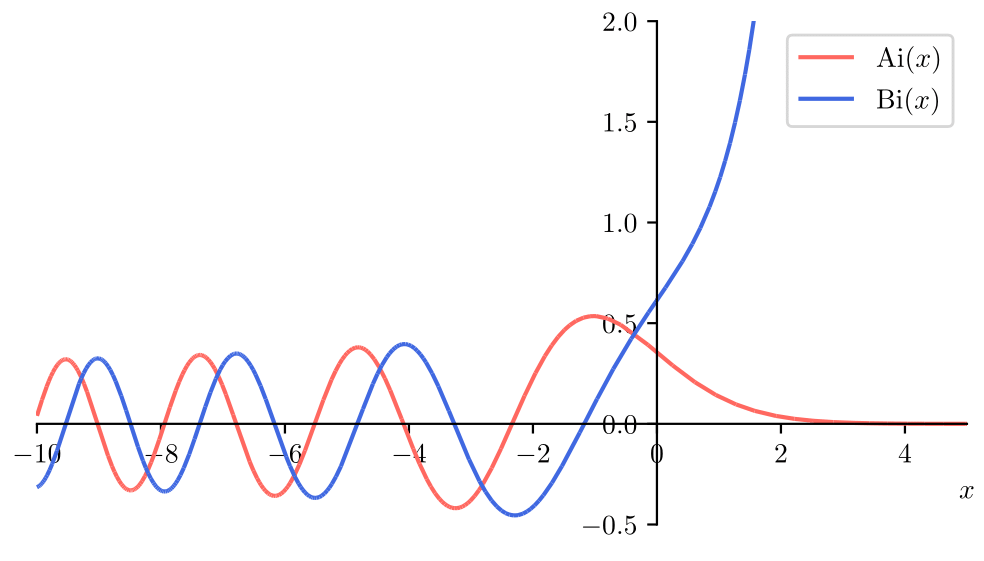
\includegraphics[width=62mm]{../fig/airy.png}
\end{minipage}
\end{figure}

である。両者をまとめてAiry関数と呼ぶこともある。
Airy関数は光学の回折理論や量子力学のWKB近似などさまざまな分野で姿を現す特殊関数である。
なおAiryとはイギリスの天文学者G.B.Airyのことであるが、Biryはただの洒落である。
}
。
\begin{numcases}{y = }
    \sqrt{x} \[ c_1 I_{\frac{1}{3}} \( \frac{2}{3} x^{\frac{3}{2}} \) 
		+ c_2 I_{-\frac{1}{3}} \(  \frac{2}{3} x^{\frac{3}{2}}\) \]
	& $(x\geq 0)$ \label{eq:Q4-3-sol-1}\\
    \sqrt{-x} \[ -c_1 J_{\frac{1}{3}} \( \frac{2}{3} (-x)^{\frac{3}{2}} \) 
		+ c_2 J_{-\frac{1}{3}} \(  \frac{2}{3} (-x)^{\frac{3}{2}}\) \]
	& $(x\leq 0)$ \label{eq:Q4-3-sol-2}
\end{numcases}

\newpage
\Q{4}{4}{3次元井戸型ポテンシャル}

次の3次元井戸型ポテンシャルのSchr\"{o}dinger方程式について考える。
\begin{equation}\label{eq:Q4-4}
  \[ -\frac{\hbar^2}{2m} \Delta + V(r) \] \psi (r, \theta, \varphi) = E \psi (r, \theta, \varphi) , \qquad V(r) = 
  \left\{
  \begin{alignedat}{2}
    &0 &\qquad& (r < a) \\
    &\infty & & (r>a)
  \end{alignedat}
  \right.
\end{equation}
ただし球座標系$(r,\theta, \varphi)$におけるラプラシアンは次の通りである。
\begin{equation}
  \Delta = \frac{1}{r^2} \frac{\6}{\6 r} \( r^2 \frac{\6}{\6 r} \) 
	+ \frac{1}{r^2\sin\theta} \frac{\6}{\6\theta} \( \sin\theta \frac{\6}{\6\theta} \)
	+ \frac{1}{r^2\sin^2\theta} \frac{\6^2}{\6\varphi^2}
\end{equation}
なお量子力学の理論から、つぎの境界条件が要請される。
\begin{numcases}{}
  r<a において \psi(r, \theta, \varphi) が有限である & \label{eq:Q4-4-boundary-1} \\
  \psi(a, \theta, \varphi)=0 & \label{eq:Q4-4-boundary-2}
\end{numcases}


\vspace{12pt}
(a). $r>a$の領域では$\psi(r, \theta, \varphi) = 0$となるので、
$r<a$の領域のみ考えればよい。このとき、
$\psi(r, \theta, \varphi) = R(r) Y(\theta, \varphi)$とおいて
方程式\eqref{eq:Q4-4}を変数分離すると次のように書けることを示せ。
\begin{align}
  - \[ \frac{1}{\sin\theta} \frac{\6}{\6\theta} \( \sin\theta \frac{\6}{\6\theta} \)
	+ \frac{1}{\sin^2\theta} \frac{\6^2}{\6 \varphi^2} \] Y (\theta, \varphi) 
		&= l(l+1) \ Y (\theta, \varphi) \label{eq:Q4-4(a)-1} \\
  \[ \frac{1}{r^2} \dr{} \( r^2 \dr{} \) 
		+ \left\{ \frac{2mE}{\hbar^2} - \frac{l(l+1)}{r^2} \right\} \] R(r) &= 0
	\label{eq:Q4-4(a)-2}
\end{align}

\vspace{6pt}
方程式\eqref{eq:Q4-4(a)-1}は球面調和関数の微分方程式であり、
$\varphi$について一価、および$\theta=0, \pi$において有限であるという条件を課せば、
$\theta, \varphi$について規格化された解は次のようになる。
\begin{equation}
  Y(\theta, \varphi) = Y_{lm} (\theta, \varphi) \qquad 
  \(
  \begin{array}{c}
    l=0, 1, 2, \dots\\
    -l \leq m \leq l
  \end{array}
  \)
\end{equation}

\vspace{6pt}
(b). 方程式\eqref{eq:Q4-4(a)-2}は球Bessel微分方程式であり、
基本解は$j_l\( \frac{\sqrt{2mE}}{\hbar} r \)$と$n_l\( \frac{\sqrt{2mE}}{\hbar} r \)$である。
いま$l$次の球Bessel関数の正の零点を小さい順に$\alpha_{l1}, \alpha_{l2}, \dots$とする。
境界条件\eqref{eq:Q4-4-boundary-1}, \eqref{eq:Q4-4-boundary-2}を要請すると、
方程式\eqref{eq:Q4-4(a)-2}の基本解が規格化定数を除いて次の関数に限られることを示せ。
\begin{equation} \label{eq:Q4-4(b)}
  R(r) = j_l\( \frac{\alpha_{ln}}{a} r \) \qquad 
  \(
  \begin{array}{c}
    n=1, 2, \dots \\
    l = 0, 1, 2, \dots
  \end{array}
  \)
\end{equation}

\vspace{6pt}
(c). 最後に解\eqref{eq:Q4-4(b)}を$r$について規格化し、
波動関数およびエネルギー固有値が次のようになることを示せ。
\begin{equation}
  \psi_{nlm} (r, \theta, \varphi) = \sqrt{\frac{2}{a^3 \[ j_{l+1}(\alpha_{ln}) \]^2 }}
	j_l\( \frac{\alpha_{ln}}{a} r \) Y_{lm} (\theta, \varphi) , \qquad
  E_{nl} = \frac{\hbar^2 \alpha_{ln}^2}{2ma^2} \qquad
    \(
  \begin{array}{l}
    n=1, 2, \dots \\
    l = 0, 1, 2, \dots \\
    -l \leq m \leq l
  \end{array}
  \)
\end{equation}

\end{document}